\chapter{Quality and Innovation}
\label{ch:qi}


\textcolor{red}{Esto puede ir probablemente como apéndice, aunque desde el punto de vista político convendría dejarlo como capítulo, tengo que reveer cómo juntar en uno calidad e innovación simultáneamente. Lo tuve que resumir muchísimo para que no sea una pesadez de lleer. Otra opción sería meter conclusiones principales desde el punto de vista innov y quality management in processes, eg. outputs check within the quality system of the institution and colaborators, periodic revision of objectives and results, etc. And then just mention that innovation and quality management were taken into account, and refere the reader to a web page containing the works produced during the thesis (in spanish, the ones I already have.). This would reduce significantly this section but would show that we took into account what we learn during the different courses. TO DISCUSS WITH ALE}

From the point of view of quality and innovation this thesis must be thought from the main outputs to the laboratory, which will be the main receipt of its developments. It is important to remember that expenditures on R \& D are a capital formation activity, i.e. investment 
\cite[Foreword]{frascati}. And in today\'s world this is one of the formost pillars in the development of countries and technology economies. It is my strong believe that the development of cutting edge technologies should be one of the goals of our society, and should result in an improvement of the lives of our countryman. 

We include the quality and innovation (Q \& I)) studie at the end, mostly because it is not easy to discuss it without the context of the research and development (R \& D) already explained. And becomes clearer if we do not have to explain the develpments and the Q \& I simultaneously. Nedless to state, that the following was taken into account on the initial steps of the R \& D process, and updated during the course of this thesis.

The initial objective of the thesis was quite large, \textit{to study and develop methods to determine, measure and apply thermoelectric properties of quantum Hall states with application to metrology. } As we have dicussed during the text, we focused on Corbino devices resulting in 
\begin{enumerate}\label{enum:developments}
    \item Gradient temperature determination by measuring and modeling the system.
    \item Thermopower measurements.
    \item Thermopower modeling.
    \item Thermal current modeling.
\end{enumerate}

The gradient temperature determination presented provides a way to determine such gradient by means of a calibrated sensor in a different section of the system, but relies on it. Also, this was proven to work in a cold-finger system, its use in a wet system could be problematic (see \ref{ch:exp} \textcolor{red}{tal vez citar párrafo específico}).

From the point of view of determine absolute temperatures on the system, there is also cavits. The method described in \ref{ch:temperature_corbino} can be applied to obtain a \textbf{relative} temperature change of the system (2DES). It is not possible from it to provide an absolute value of temperature. But, importantly, such change it is very important too, since the calibrated sensor is not determing the actual temperature of the 2DES (system to measure), not even the crystal temperature containing it. It provides then, a mean to measure temperature changes during measurements. 

The thermopower measurements provided two main outputs: the development of high resolution measurements and unexpected behaivour of the 2DES under the QH \textcolor{red}{incluir QH en glossary} state. 

The thermopower modeling resulted in a model \ref{ch:vtp_g_model} that describes the system in the semi-filled LL and returns a value for the temperature gradient obtained 
\footnote{This gradients corresponds to the AC responses. In the model \ref{ch:vtp_g_model} and experimental \ref{ch:vtp_g_model} sections further explanation of this important detail are given.}.
As we have discussed the measured thermopower in and out of phase was not expected, not even its maximum values. We were able to produce a model that at least provides an explanation of these behaviors, based on the measurements.

Finally the semi-filled LL model was further developed to predict the thermal currents of the systems. From the model point of view, it predicts a very interesting behiviour, that could be exploited to cool down sections of a system. This yet remains to be experimentally proven.

All itemized cases fulfill the cryteria to be considered an R \& D activity. They have benn proven to be \textit{novel}, since all of them have been peer reviewd and published, \textit{creative} the results and models produced are not obvious and resulted in possible new applications (cooling). As most cutting edge studies they result to be \textit{uncertain}, we new we were able to produce devices and measurements, but by no means we were expecting several outcomes that we have described. As always in science, and specially in metrology we have produced very \textit{systematic} studies, that are also \textit{reproducible} between laboratories (Argentine and Switzerland) and devices. So the basis of our studies comply with all requirements of R \& D.

Stablished this, we can analize the threats and opportunities of the project (context). By using a innovation management tool and taking into account any thinkable possible theat and opportunitie both internal or external (macro and micro), we produced a scheme resuming such posibilities \ref{fig:innov-theats_opportinities}. This figure also includes some possible scenarios, that resulted to be out-of context. 

\begin{figure}
    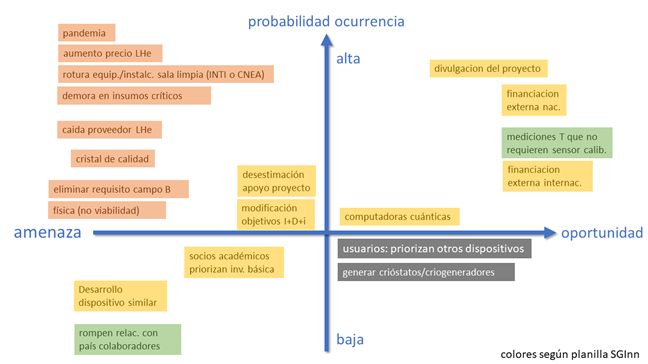
\includegraphics[width=0.9\textwidth]{figures/innovation/theatsOpportunitiesInnov.png}
    \caption{Opportunities and threats of the project, they are plotted against its degree of occurrence probability. Their resulting score is given by color, being redish a high-priority, yellow mid-priority and green low-priority theats. Meanwile high priority opportunities are green, yellow mid priority and finally grey resulted in out of context opportinities.}
    \label{fig:innov-theats_opportinities}
\end{figure}

For each one of this possible factors a possible solution-alternative and course of action was evaluated. We will not indicate each one of them, but for example, it is usual that the micro-machining facilities find working problems that could result in heavy delays in our goals. To overcome such possibilities we had the chance to work in two near facilities (INTI and CNEA). This was a very interesting situation, since it resulted in a nice flexibility at the time to produce our devices.

\section{Interested Parties}
\label{sec:interested_parties}

As in context, the interested parties were studied by Q \& I tools. One important point is that this project was self generated, and that the temperature determination of the systems is to be use in the Quantum Standards Laboratory. But, any possible development in this regard could be implemented in other institutes working on cryogenic measurements under magnetic fields. There are superior tecnologies, but its implementation and development (most not comercial) would require long development times, cyostat modifications and clean room facilities not easely accesible, e.g. Johnson noise thermometry \cite{Johnson1928,nyquist1928,qu2019johnson} that would imply the development from scratch of such tecnology in our laboratory 
\footnote{This being said, is my firm believe that our institute should start steps forward this technology in the comming years, it is becoming a standard \cite{flowers2017boltzmann,Department2013}.}.

Commercial resistive and semiconducting sensors are available for cyogenic systems, most of them are quite large, very expensive (particularly the calibrated ones) and they do not provide the 2DES temperature, they measure usually some part of our cyosystem. Any group working with high fields and low temperatures could become interested in any tecnology providing the kind of measurment developed in this thesis.

The interested parties are detailed in \ref{fig:innov-interested-parties}, from the analisys tools we obtain that the local and external research groups present no applicable action, the same happens regarding cryogenic companies. En both cases the influece power is big but the interest at this time is low, the only way to improve this is to obtain a working prototype to develop specific actions.
Since the development is to be applied in a national institution, the Nation is represented as an Argentine map, which supports the development and the institutions undertaing it. It is a group which influence power is high but its interest for now very low.  Because of this its participation should be kept and must be informed in the best way possible. There are only scarse cases wne this group increses its interest, a good positive example are the innovations and research regarding COVID19, satellites (in is final lounch stage), and such. 

Of course our collaborators (national and international) are one of the main influece parties, resulting to be in the direct interest group, in the same way as the national institutions involved, like INTI, UNSAM and the parties directly involved in the develpment of this thesis.
The case of INCALIN-UNSAM is double, since its aim is to increse local develpments and to show how research, quality and innovation can be applied to local cutting edge technologies.

\begin{figure}
    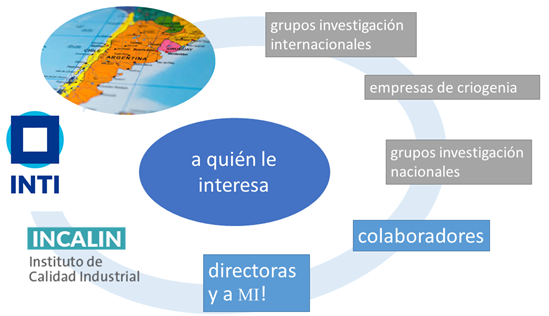
\includegraphics[width=0.8\textwidth]{figures/innovation/interested-parties.png}
    \caption{Small schematic figure indicating the evaluated possible interested parties by means of the quality and innovation tools used.}
    \label{fig:innov-interested-parties}
\end{figure}

Given all what we have discussed, and the usual technology readiness level scales, see Fig.~{fig:innov-trl}, we can set scales for the developments itemized initially~\ref{enum:developments}
\begin{figure}
    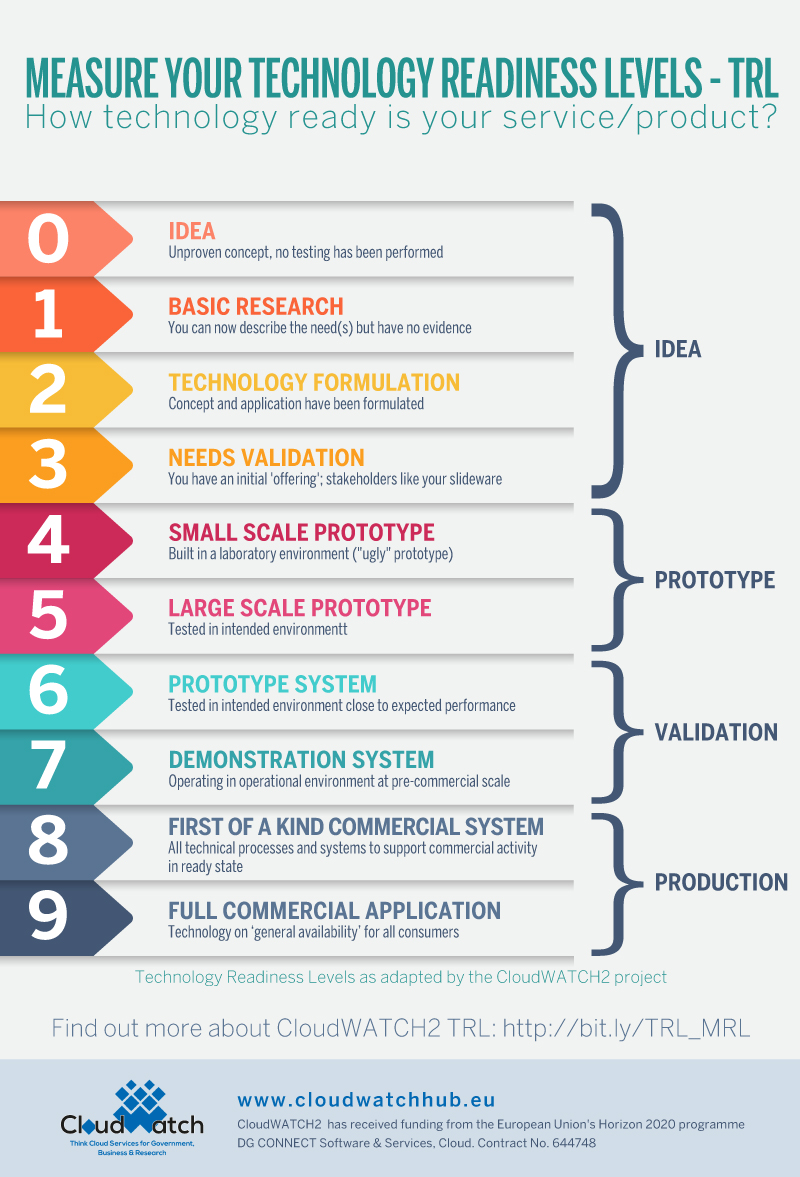
\includegraphics[width=0.8\textwidth]{figures/innovation/trl.jpg}
    \caption{\textcolor{red}{tengo que hacer el propio}}
    \label{fig:innov-trl}
\end{figure}


\textcolor{red}{citar: \cite{frascati,osloManual,pmbok2021guide}}

\textcolor{red}{Incluir acá o en la sección inicial \url{https://www.bipm.org/documents/20126/43742162/CIPM-MRA-G-13.pdf/f8b8c429-42e0-4cf1-dc6c-bc60ab7f371a} y \url{https://www.bipm.org/documents/20126/43742162/CIPM-MRA-P-11.pdf/} Donde se explica el MRA, esto es hyper relevante respecto a cómo impactamos. Desde el punto de vista del MRA, toda mejora va relacionada directamente a las CMCs declaradas de Argentina. De esto hablé un poco en el trabajo de Calidad enfocada a procesos, no lo incluí acá aún. En esa misma dirección habría que incluir la ISO 17025 }




